\documentclass[12pt, a4paper, oneside]{book}

% Language setting
\usepackage[english]{babel}
\usepackage{setspace}
% Set page size and margins
% Replace `letterpaper' with `a4paper' for UK/EU standard size
\usepackage[a4paper,top=2cm,bottom=2cm,left=3cm,right=3cm,marginparwidth=1.75cm]{geometry}

% Useful packages
\usepackage{amsmath}
\usepackage{graphicx}
\usepackage[colorlinks=true, allcolors=blue]{hyperref}

\usepackage{csquotes}

\usepackage{float}
\usepackage{fix-cm}
\usepackage[table]{xcolor}
\usepackage{titlesec}
\usepackage{soul, color}
\definecolor{gray75}{gray}{0.75}
\newcommand{\hsp}{\hspace{0pt}}
\titleformat{\chapter}[hang]{\flushright
\fontseries{b}\fontsize{80}{100}\selectfont}{\fontseries{b}\fontsize{100}{130}\selectfont \textcolor{gray75}\thechapter\hsp}{0pt}{\Huge\bfseries}[]

\usepackage{tabularx}

\title{DevOps, Software Evolution and Software Maintenance, BSc (Spring 2024)}
\author{Course code: BSDSESM1KU}




\begin{document}
\begin{spacing}{1.5}

\begin{minipage}{\textwidth}
\maketitle

\begin{center}
    Exam Assignment by: \\
    \hfill \break
    \bgroup
    \def\arraystretch{1.5}%
    \begin{tabularx}{0.8\textwidth} { 
      | >{\centering\arraybackslash}X 
      | >{\centering\arraybackslash}X | }
     \hline
     \cellcolor[HTML]{EFEFEF} Student & \cellcolor[HTML]{EFEFEF} Email \\
     \hline
     Daria Damian & dard@itu.dk \\
     \hline
     Hallgrímur Jónas Jensson & hajj@itu.dk \\
    \hline
     Mathias E. L. Rasmussen & memr@itu.dk \\
    \hline
     Max-Emil Smith Thorius & maxt@itu.dk \\
    \hline
    Fujie Mei & fume@itu.dk \\
    \hline
    \end{tabularx}
    \egroup
\end{center}
\end{minipage}

\tableofcontents

\chapter{System's Perspective}

\section{Design and architecture of the Minitwit system}


ITU-MiniTwit is designed as a microservices architecture, leveraging containerization to ensure isolation, ease of deployment, and scalability. The system's architecture facilitates independent development and service deployment, enhancing maintenance and testing capabilities.
\begin{figure}[h]
    \centering
    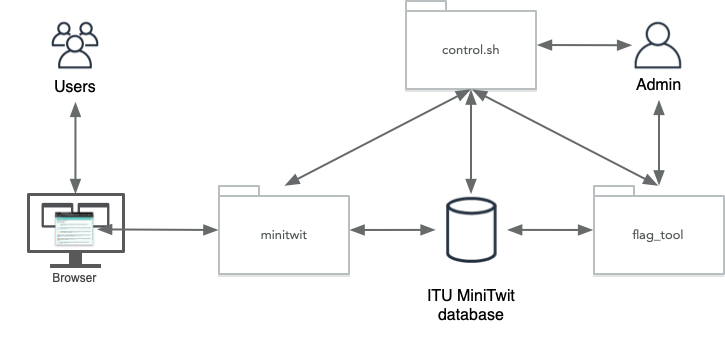
\includegraphics[width=\textwidth]{images/ITU-minitwit-architecture.png}
    \caption{High-level ITU-MiniTwit architexture}
\end{figure}\\

Detailed Architecture:

\begin{itemize}

\item API Service:

    \subitem Function: Handles all client-server interactions, processing client requests and sending responses back to clients.
    \subitem Implementation: Implemented using Go, which is suitable for creating performant and scalable backend services.
    \subitem Files: Located within the API directory, which contains all the routing and logic for handling HTTP requests.
\item Database Service:
    \subitem Function: Manages data storage and retrieval, serving as the persistent storage layer for the application.
    \subitem Implementation: Utilizes SQL, making use of relational database management systems.
    \subitem Files: The database directory contains scripts and configurations for database setup and management.
\item Front-end:
    \subitem Function: Provides the user interface through which users interact with the ITU-MiniTwit application.
    \subitem Implementation: Usage of HTML, CSS, and JavaScript files served by the Python service.
    \subitem Files: included in the root directory that contains HTML templates and JavaScript files.
\item Containerization and Orchestration:

    \subitem Utilizes Docker to containerize the application components, ensuring that each component runs in an isolated environment with its dependencies.
    \subitem Docker Compose helps in defining and running multi-container Docker applications, where services such as the API and database are orchestrated to work together.
\end{itemize}


\section{Dependencies of the Minitwit system}


This section will detail all the technologies, tools, and external services our system depends on, structured into categories for clarity.

1. Development Dependencies

\begin{itemize}
 
\item   Programming Languages:
    \subitem   Python: Used for writing backend logic, potentially for web serving and scripting tasks. Dependencies are managed via requirements.txt, which includes libraries for web frameworks, database integration, etc.
    \subitem Go: Employed for building efficient, compiled services, possibly for high-performance backend components. 
\item Version Control:
    \subitem Git: Essential for source code management, allowing version control and collaboration among developers.
    \subitem GitHub: Hosts the repository and provides additional tools for code reviews, issue tracking, and GitHub Actions for CI/CD.

\item Local Development Environment:
    \subitem Vagrant: Used to configure and manage virtual development environments that mirror the production environment, ensuring consistency across different machines.
    \subitem Docker: Provides a containerized environment to run services isolated from the host system, facilitating easier setup and dependency management.


\item External APIs and Services:
    \subitem Graphana?
    \subitem Prometheus: Employed for monitoring the application’s performance metrics, helping in proactive management and optimization of the application performance.
\end{itemize}

2. Build and Deployment Dependencies
Tools and technologies used to build, test, and deploy the ITU-MiniTwit application.

\begin{itemize}

\item Build Tools such as Makefile: Automates the compilation and building process, allowing developers to run predefined scripts for building the application, running tests, and other tasks with simple commands.
\item Continuous Integration/Continuous Deployment (CI/CD) such as GitHub Actions: Automates the workflow of code integration, testing, and deployment whenever the repository is updated, ensuring that new code changes integrate smoothly and deploy automatically.
\item Container Orchestration such as Docker Compose: Manages multi-container Docker applications, used in development and production to configure and orchestrate multiple services (API, database, etc.) to work together seamlessly.
    
\end{itemize}

3. Runtime Dependencies

\begin{itemize}

\item Server Environment:
\subitem Docker
\subitem Linux/Unix: The underlying operating system for servers running Docker containers, providing robustness and stability.
\item Database Management: SQL Database: Our application uses an SQL database for data persistence, and for database operations and management.

\end{itemize}

\begin{figure}[h]
    \centering
    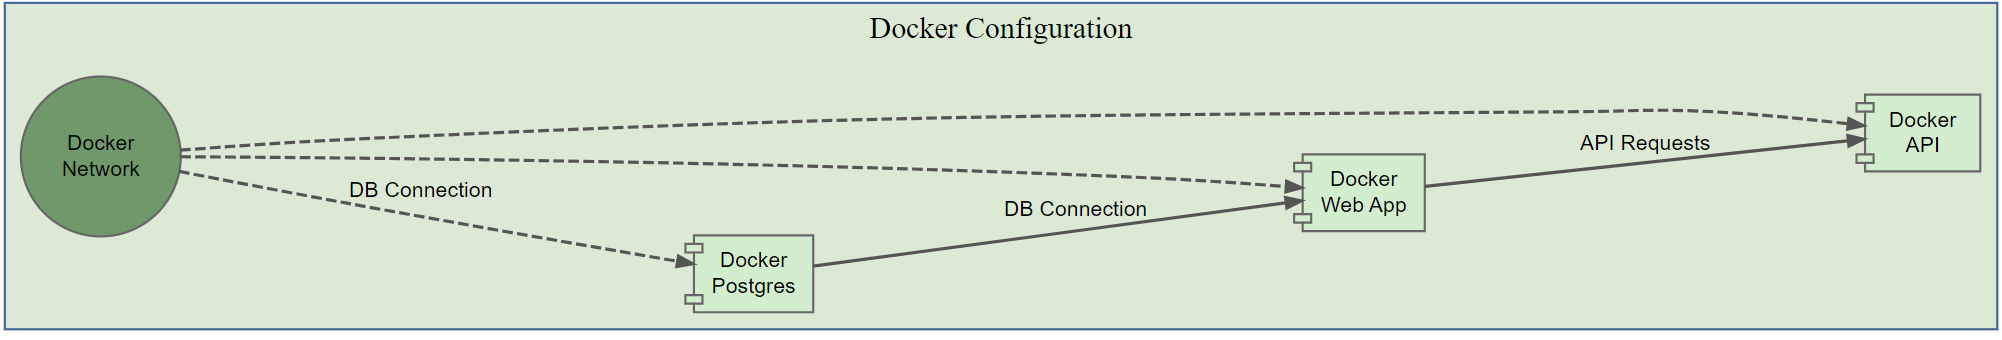
\includegraphics[width=\textwidth]{images/dockerconfig.png}
    \caption{Docker Configuration}
\end{figure}


\section{Important interactions of subsystems}

\subsubsection{Information Flow in UML ITU-MiniTwit:}

link for the UML diagrams: \href{https://drive.google.com/file/d/1xU3Uf7EZC5fq4Bzw-O73jOwjMg971a8d/view?usp=sharing}{link1},\href{https://drive.google.com/file/d/1vgYJsYiDPGsxxs7oxMblu9runmONP_LT/view?usp=sharing}{link2}

\begin{figure}[H]
    \centering
    \fbox{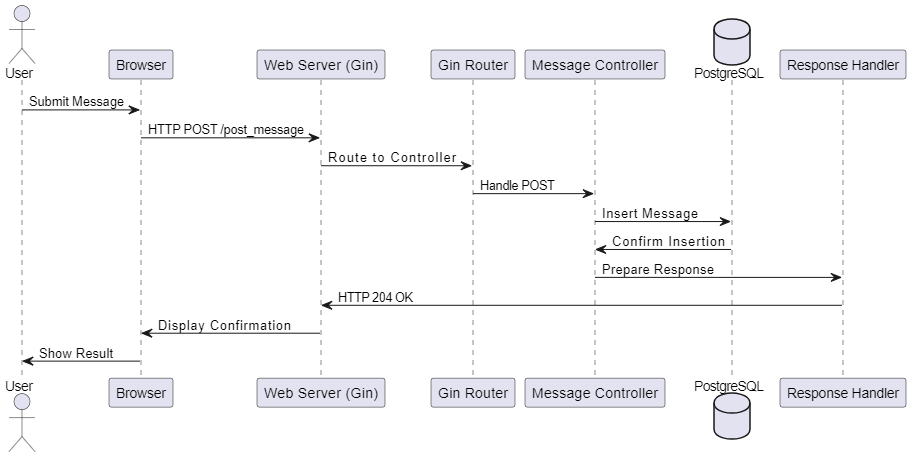
\includegraphics[width=\textwidth]{images/uml1.drawio.png}}
    \caption{Information Flow - UML Sequence diagram}
    
\end{figure}

\newpage
\begin{figure}[H]
    \centering
    \fbox{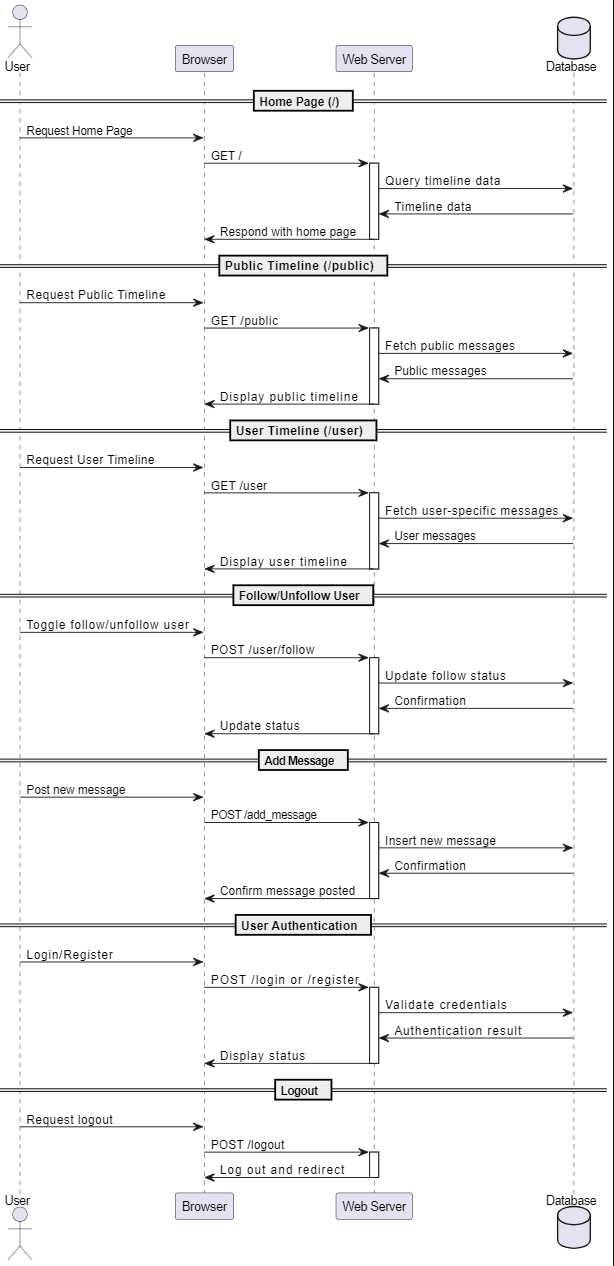
\includegraphics[width=0.8\textwidth]{images/UML2.drawio.png}}
    \caption{How requests from the simulator traverse your system}
    
\end{figure}

\section{Current state of the system}
Ideas:
\begin{itemize}
    
\item Static Analysis:
\item Present results from static analysis tools to discuss code quality, potential bugs, and security issues.
\item Mention any significant findings and how they impact the overall system.
\item Quality Assessment:
\item Discuss methods used for assessing the quality of the application (e.g., code reviews, testing coverage).
\item Summarize the current quality metrics and any goals or benchmarks your team is aiming to achieve.
\item Using Prometheus, document current performance metrics of the system, analyzing aspects such as response times, system throughput, and error rates.

\end{itemize}

\begin{itemize}

    \item[1.] Static Analysis Results:
Static analysis tools examine your code without executing it to find potential issues. Here's what to look at:

\item Code Quality Metrics:
\item Complexity: Measures how complex the logic in your codebase is. Lower complexity often correlates with easier maintenance.
\item Code Style Compliance: Checks adherence to coding standards and conventions which help in maintaining code consistency.
\item Potential Bugs: Identification of code patterns that could lead to errors.
\item Code Smells: Highlight suboptimal code practices that might not cause bugs but could reduce code quality or increase complexity.
\item Security Vulnerabilities:
\item Known Vulnerabilities: List of known vulnerabilities in your dependencies or your code that could be exploited.
\item Security Hotspots: Areas in the code that require a manual review to ensure they are secure.
\item[2.] Quality Assessments:
Quality assessments go beyond static code analysis by incorporating other factors such as unit test coverage and integration test results.


\item Test Coverage:
\item Unit Test Coverage: Percentage of your codebase covered by unit tests. High coverage can reduce the likelihood of bugs making it to production.
\item Integration Test Results: These tests cover interactions between modules or services and help identify issues in the way components integrate.
\item Performance Metrics:
\item Response Times: Average time it takes for your system to respond to user actions.
Resource Usage: Usage statistics for CPU, memory, and other resources. High usage might indicate a need for optimization.
\item Dependency Health:
\item Outdated Libraries: Using outdated libraries can expose your system to security vulnerabilities and compatibility issues.
License Compliance: Ensuring that all library licenses comply with your project's licensing.
\item 3. System Observability and Monitoring:
Logs Analysis: Insights into errors and unusual system behavior captured in logs.
Metrics Dashboard: A real-time dashboard showing key performance metrics.
Alerts History: Review of past alerts to understand recurring issues or spikes in resource usage.
\item 4. Development Practices:
Code Review Practices: Regular code reviews help maintain code quality and mentor junior developers.
Build and Deployment Frequency: Frequency of deployments can indicate the agility and health of the development process.
Feature Development Speed: How quickly new features move from conception to production
% A description and illustration of the:
% - Design and architecture of your ITU-MiniTwit systems
% - All dependencies of your ITU-MiniTwit systems on all levels of abstraction and development stages. That is, list and briefly describe all technologies and tools you applied and depend on.
% - Important interactions of subsystems
%    - For example, via an illustrative UML Sequence diagram that shows the flow of information through your system from user request in the browser, over all subsystems, hitting the database, and a response that is returned to the user.
%    1- Similarly, another illustrative sequence diagram that shows how requests from the simulator traverse your system.
% - Describe the current state of your systems, for example using results of static analysis and quality assessments.
\end{itemize}


\chapter{Process' perspective}
% This perspective should clarify how code or other artifacts come from idea into the running system and everything that happens on the way.
% In particular, the following descriptions should be included:
% - A complete description of stages and tools included in the CI/CD chains, including deployment and release of your systems.
% - How do you monitor your systems and what precisely do you monitor?
% - What do you log in your systems and how do you aggregate logs?
% - Brief results of the security assessment and brief description of how did you harden the security of your system based on the analysis
% - Applied strategy for scaling and upgrades
% In case you have used AI-assistants during your project briefly explain which system(s) you used during the project and reflect how it supported/hindered your process.

\section{CI/CD Chain}
We implemented a GitHub Actions workflow to automate the process of testing, building and deploying the most recent version of Minitwit. It is set to execute on each push to the 'Main' branch of our GitHub repository. The workflow is separated into three main jobs: 'BuildAndTest', 'Deploy', and 'Release' which are executed sequentially, each dependent on the last executing successfully.

\subsection{Triggers}
The workflow is triggered on two specific GitHub events: manual triggers via workflow\_dispatch and on pull requests to the main branch. 

\subsection{Jobs}
\subsubsection{BuildAndTest}
In this step all relevant images are built and pushed to the Docker hub and then run and tested to ensure that the system will work as expected. The key steps are as follows:

\begin{enumerate}
    \item \textbf{Checkout:} 
    \begin{itemize}
        \item Uses \texttt{actions/checkout@v2} to fetch the codebase from the repository.
    \end{itemize}
    
    \item \textbf{Environment Setup:} 
    \begin{itemize}
        \item Dynamically creates a \texttt{.env} file with database configurations sourced from GitHub secrets.
    \end{itemize}
    
    \item \textbf{Docker Operations:}
    \begin{itemize}
        \item Logs into Docker Hub using credentials from GitHub secrets to push built images.
        \item Builds and pushes multiple Docker images, including:
        \begin{itemize}
            \item The application image
            \item API image
            \item A test database image
        \end{itemize}
    \end{itemize}
    
    \item \textbf{Python Setup and Dependency Installation:}
    \begin{itemize}
        \item Configures the Python environment.
        \item Installs necessary dependencies to ensure consistent testing conditions.
    \end{itemize}
    
    \item \textbf{Testing:}
    \begin{itemize}
        \item Executes integration tests by setting up the application and its dependencies in Docker containers.
        \item Conducts API tests and application-specific tests to ensure functionality and reliability.
    \end{itemize}
\end{enumerate}

\subsubsection{Deploy}
The \textbf{Deploy} job is activated on successfully completing the \textbf{BuildAndTest} job. This job manages the deployment of the application to the remote server where the application is hosted. The steps are:

\begin{enumerate}
    \item \textbf{Checkout:} 
    \begin{itemize}
        \item Retrieves the latest codebase from the repository, uses \texttt{actions/checkout@v2} similar to the first job.
    \end{itemize}
    
    \item \textbf{SSH Configuration:} 
    \begin{itemize}
        \item Prepares SSH keys to establish a secure connection to the deployment server.
    \end{itemize}
    
    \item \textbf{Deployment Execution:}
    \begin{itemize}
        \item Updates environmental configurations and transfers necessary files to the server using SSH.
        \item Employs Docker Compose on the server to pull the latest Docker images.
        \item Deploys the images using Docker Stack, which effectively updates the running application on the server.
    \end{itemize}
\end{enumerate}

 \subsubsection{Release}
 After the previous jobs have been successfully completed, this job manages software versioning and public release.

 \begin{enumerate}
    \item \textbf{Version Calculation:}
    \begin{itemize}
        \item Executes a script to determine the new version number for automated version tracking.
    \end{itemize}
    
    \item \textbf{GitHub Release Creation:}
    \begin{itemize}
        \item Uses \texttt{actions/create-release@v1} to create a formal release on GitHub.
        \item Tags the release with the new version number and provides release notes outlining the changes in this version.
    \end{itemize}
\end{enumerate}



\section{Monitoring}
For monitoring we use Prometheus to collect metrics, and integrate with Grafana for live visualization of key metrics. We have two dashboards, one monitoring the API and the other the database.

\subsection{API dashboard}
 \begin{enumerate}
    \item \textbf{Response time:}
    This chart displays the response times of requests over the past six hours, with separate lines for the slowest 95th and 99th percentile requests.

    \item \textbf{Rate of HTTP requests:}
    Shows the number of HTTP requests per second, categorized by endpoints.
    
    \item \textbf{HTTP Requests Total:}
    Shows the total number of HTTP requests received, categorized by endpoints.
    
    \item \textbf{Total HTTP request errors:}
    Shows a chart of total HTTP request errors by endpoint.
    
    \item \textbf{Bad HTTP request total:}
    Shows the total number of bad requests made, by endpoint.
\end{enumerate}

\subsection{Database dashboard}
 \begin{enumerate}
    \item \textbf{Amount of users:}
    Gauge charting user count.
    
    \item \textbf{Amount of messages:}
    Gauge charting message count.    
    \item \textbf{Amount of follows:}
    Gauge charting count of follows between users.
    
    \item \textbf{Distribution of users by message count:}
    Bar chart showing count of users by number of messages.
    \item \textbf{Distribution of users by following count:}
    Bar chart showing count of users by how many they follow.
\end{enumerate}



\section{Logging}
In the figure below, you can see how our ELKB stack is structured to ship logs to Elasticsearch and further analyze them.
\begin{figure}[H]
    \centering
    \hbox{\hspace{-8em}
    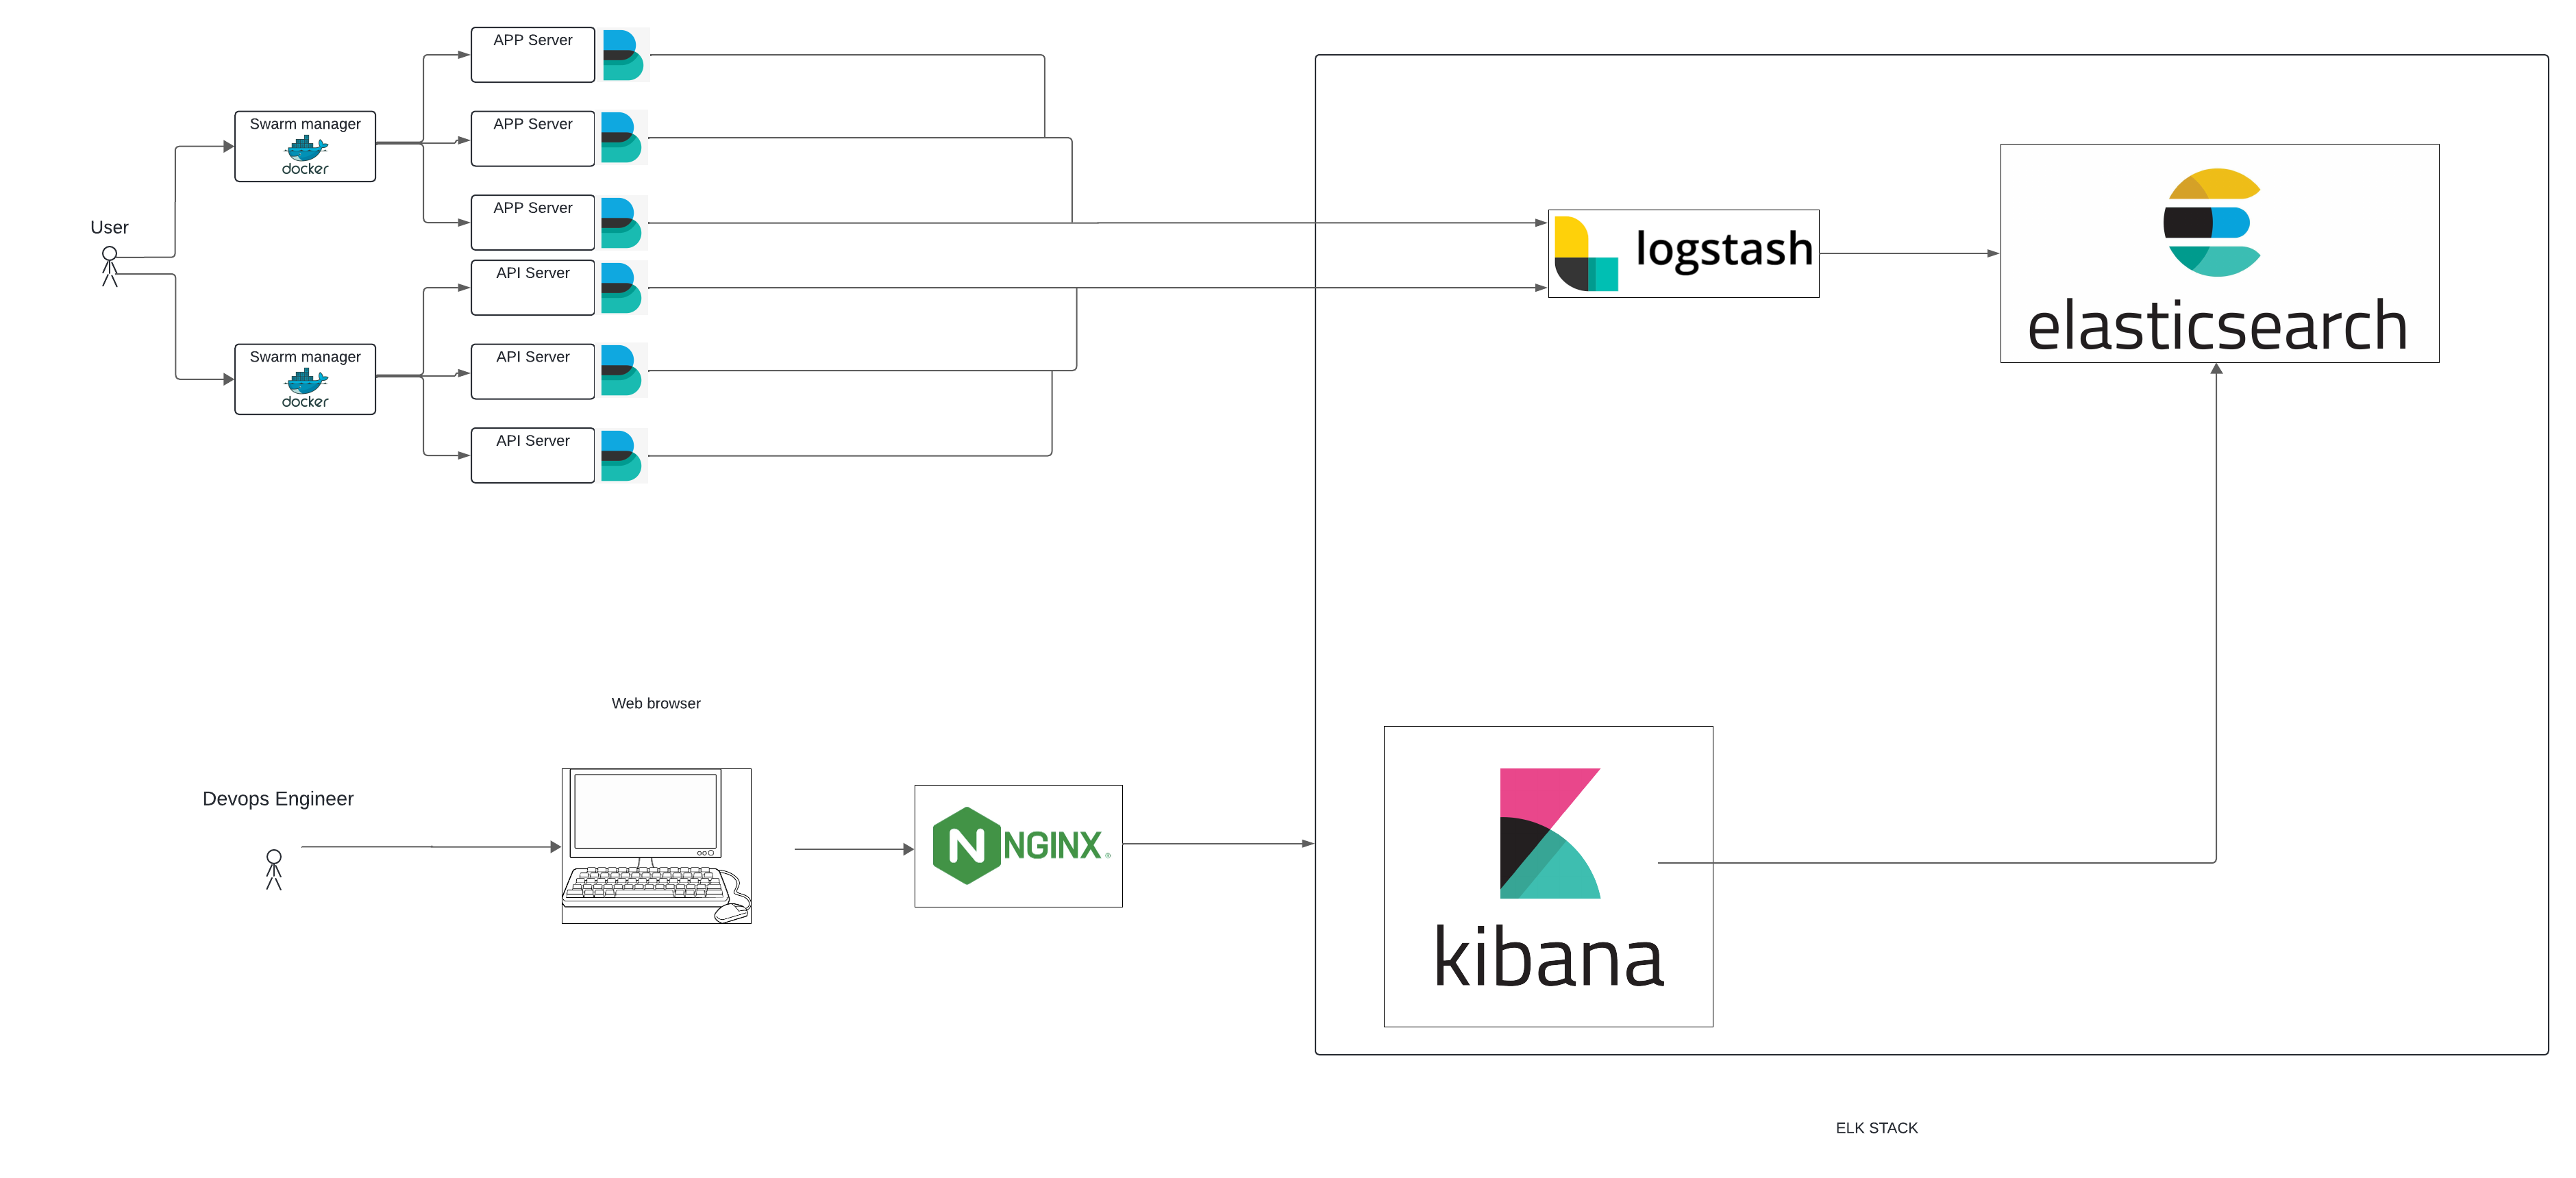
\includegraphics[scale = 0.35]{images/elk.png}}
    \caption{ELK stack}
    \label{fig:elk-stack}
\end{figure}

What enables the Filebeat to ship logs is a label tag added to our "app" and "api" services which enables Filebeat to autodiscover logs from those containers which has that option enabled. Filebeat will collect logs only containing a timestamp, which are those generated by the logger of our code, and ship them to Logstash where they will be further processed to be outputted to Elasticsearch. Finally, and Devops engineer can analyze and visualize this logs through Kibana through their browser, where the stack will be reversed proxied by Nginx for authentication reasons. \bigskip

What we log in our application is the main events that occurs, we mainly use 4 levels for this purpose: info, debug, error and fatal. We used "info" level to communicate the events in a general level of how things are happening; "debug" for debugging purposes, how parameters are being changed and passed; "error" when the program encounters some non-fatal errors for example in our Go app when the "err" parameter is not nil we notify it with the error level; and finally "fatal" is used for errors that halts or crashes the application. \bigskip

All logs are collected in a single index pattern, from all sources from the "app" and "application. We can distinguish the sources in Kibana because you can see from which folder and which file is the log generated from. Please, see image below:
\begin{figure}
    \centering
    \hbox{\hspace{-5em}
    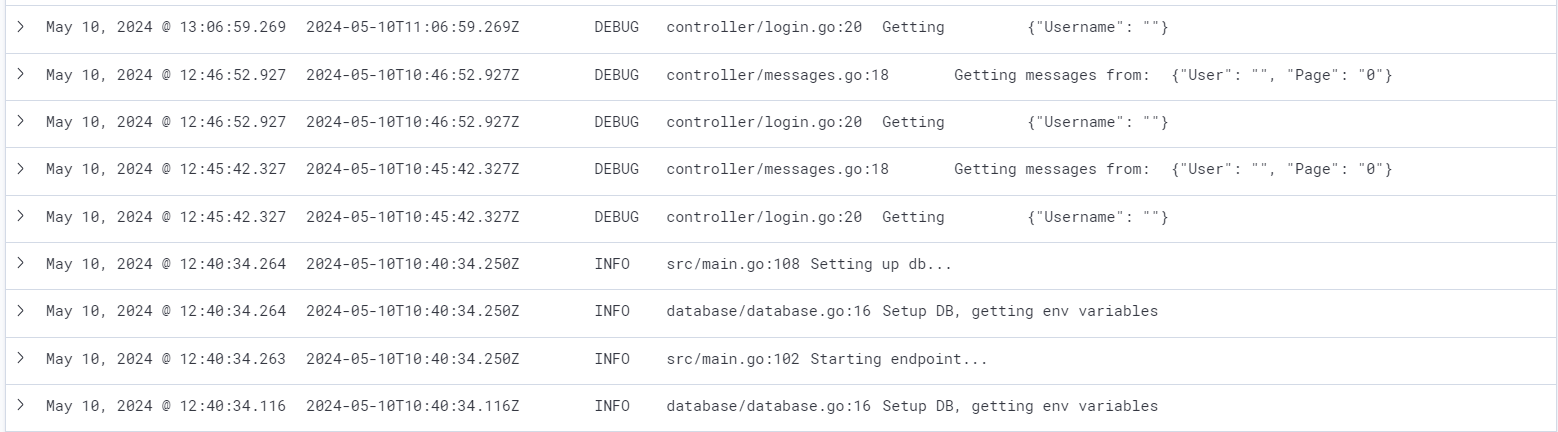
\includegraphics[scale = 0.6]{images/kibana.png}}
    \caption{Logs from Kibana}
    \label{fig:kabana-logs}
\end{figure}
\section{Security assessment}

\section{Scaling strategy}

\chapter{Lessons Learned Perspective}

\section{Evolution and refactoring}

\section{Operation}

\section{Maintenance}

% Describe the biggest issues, how you solved them, and which are major lessons learned with regards to:
% - evolution and refactoring
% - operation, and
% - maintenance
% of your ITU-MiniTwit systems. Link back to respective commit messages, issues, tickets, etc. to illustrate these.
% Also reflect and describe what was the "DevOps" style of your work. For example, what did you do differently to previous development projects and how did it work?

Lorem ipsum dolor sit amet, consectetur adipiscing elit. Donec venenatis enim a nulla molestie, ac feugiat justo egestas. Nullam interdum lorem et neque ullamcorper volutpat sed sit amet tortor. Praesent sit amet aliquet risus, et accumsan mi. Sed facilisis condimentum varius. Praesent et nunc cursus, laoreet nisi a, venenatis nisl. Integer diam magna, iaculis at dapibus et, rutrum in leo. Pellentesque feugiat diam felis, quis ornare eros dignissim et. Maecenas sed laoreet nunc. Morbi porttitor massa id dui aliquam, non ultrices dolor malesuada.

Cras et porta ex. Lorem ipsum dolor sit amet, consectetur adipiscing elit. Aliquam erat volutpat. Phasellus eget ipsum sit amet nulla porttitor rhoncus at eget elit. Aenean vulputate, urna sed lacinia luctus, sem nisi iaculis nunc, vitae mattis neque sem in felis. Sed tempor tincidunt dapibus. Morbi porta ex erat, sed ornare mi gravida nec. Phasellus ut nunc venenatis, mollis est vestibulum, laoreet nibh. Mauris in vulputate diam. Nunc ullamcorper vestibulum velit, eget volutpat leo vulputate at. Nam in tortor id dolor elementum lobortis at ut elit. Nulla in interdum mi. Sed aliquam ullamcorper blandit.
\end{spacing}

\chapter{Appendix}


\end{document}
